%----------------------------------------------------------------------------------------
%	PACKAGES AND THEMES
%----------------------------------------------------------------------------------------

\documentclass[notes]{beamer}

%Cheat-Sheet: https://www.cpt.univ-mrs.fr/~masson/latex/Beamer-appearance-cheat-sheet.pdf
\usetheme{Frankfurt}

%-- Layout --%
% font size
\usepackage[fontsize=11pt]{scrextend}
\usepackage{amsmath}
\usepackage[short]{optidef}
\usepackage[backend=bibtex,style=authoryear]{biblatex}
% page
\setbeamersize{text margin left=1cm, text margin right=1cm}
\setbeamercolor{button}{bg=blue, fg=white}
% line space 
\usepackage{setspace}
\setstretch{0.8}
% footline
\addtobeamertemplate{navigation symbols}{}{
    \usebeamerfont{footline}
    % \usebeamercolor[fg]{footline}
    \hspace{2em}
    \insertframenumber/\inserttotalframenumber    }
% headline
\setbeamercovered{transparent}

%-- Figure --%
\usepackage{graphicx}
% \usepackage{subfig}

%-- Table --%
\usepackage{tabularx,booktabs}
\newcolumntype{Y}{>{\centering\arraybackslash}X}

%-- Text --%
\usepackage{xcolor}
% \usepackage{tikz}

%-- Math --%
\usepackage{amssymb}
\usepackage{amsmath}

%-- Caption --%
\usepackage{caption}
\usepackage{subcaption}

%-- Effects --%
\usepackage{hyperref}

%----------------------------------------------------------------------------------------
%	TITLE PAGE
%----------------------------------------------------------------------------------------

\title[]{Debt Financing Strategies of Heterogeneous Firms} % The short title appears at the bottom of every slide, the full title is only on the title page

\author{Barnab\'as Sz\'ekely} % Your name

\date{\today } % Date, can be changed to a custom date

\begin{document}
\renewcommand{\arraystretch}{1.4}

\begin{frame}
\titlepage % Print the title page as the first slide
\end{frame}

%%----------------------------------------------------------------------------------------
%	PRESENTATION SLIDES
%----------------------------------------------------------------------------------------

%------------------------------------------------
\section{Intro}


\begin{frame}[label=slide2]
\frametitle{Asset-Based and Cash-Flow Based lending}

Asset-based lending (ABL):
\begin{itemize}
\item Secured against borrowers' (physical) assets
\item Financial distress is expected to be resolved by liquidation 
\item Collateral value matters
\end{itemize} \vspace{4mm}
Cash flow-based lending (CFL):
\begin{itemize}
\item No specific assets pledged as collateral: unsecured or secured against equity or the entire corporate entity 
\item Financial distress is expected to be resolved by reorganization 
\item Continuation value matters
\end{itemize}  \vspace{2mm}
\begin{center}
\hyperlink{secUnsec}{\beamerbutton{Secured vs. Unsecured}}
\end{center}
\end{frame}

%------------------------------------------------
\begin{frame}
\frametitle{Reconsidering financial frictions}
Lian and Ma (2021): 80\% of US corporate debt is CFL \vspace{5mm} \\
Model Implications
\begin{itemize}
\item ABL $\rightarrow$ asset based borrowing constraints ($b \leq \phi_k k$)
\item CFL $\rightarrow$ earnings based borrowing constraints ($b \leq \phi_\pi \pi$)
\end{itemize} \vspace{3mm} 
Credit market frictions: 
\begin{itemize}
\item Often modelled asset based constraints
\item Earnings based constraints yield different results
\item Greenwald (2019), Lian and Ma (2021), Drechsel (2023)
\end{itemize}

\end{frame}

%------------------------------------------------
\begin{frame}
\frametitle{Motivation}
Empirically, both ABL and CFL are present
\begin{itemize}
\item Not all firms have equal access: limited availability of CFL 
\item Misallocation of capital and aggregate productivity losses
\item The aggregate costs are unclear
\end{itemize} \vspace{7mm} 
Debt financing strategies determine the nature (and severity) of credit market frictions
\begin{itemize}
\item How investment decisions react to aggregate shocks
\item How firm distribution is affected
\end{itemize}

\end{frame}


%------------------------------------------------
\begin{frame}
\frametitle{Outline}
\begin{enumerate}
\item Empirical distribution of debt financing strategies \vspace{5mm} \\
\item Heterogeneous firms model with ABL and CFL in equilibrium  \vspace{5mm} \\
\item Conclusion and potential future directions
\end{enumerate} 

\end{frame}

\section{Determinants of CFL}

%------------------------------------------------
\begin{frame}[label=DandC]
\frametitle{Data and Classification}
Data: 
\begin{itemize}
\item Debt-level observations: CapitalIQ
\item Firm level observations: Compustat North America
\item Mostly US and Canadian firms - period: 2018Q1
\item Total of 32,835 debt instruments held by 4,489 NFCs
\end{itemize} \vspace{2mm}
Classification:
\begin{itemize}
\item Debt instruments are classified individually into ABL or CFL, following the approach of Lian and Ma (2021) 
\item By volume, 73.4\% of total corporate debt is CFL
\end{itemize}
Could be refined via Dealscan, Orbis and Compustat Global
\begin{center}
\hyperlink{Classification}{\beamerbutton{Classification Details}}
\end{center}
 
\end{frame}

%------------------------------------------------
\begin{frame}
\frametitle{Firm and loan level descriptive statistics}
\begin{table}[H]
\centering
\resizebox{\textwidth}{!}{%
\begin{tabular}{lrrrrrr}
\hline
\multicolumn{7}{l}{\textbf{Panel A: Firm Level Statistics}} \\
 & Mean & p10 & p25 & Median & p75 & p90 \\
\hline
Total assets (millions USD) &  1834.05 & 1.42 & 19.70 & 191.18 & 854.99 & 3269.41 \\
Number of employees (thousands) & 12.31 & 0.02 & 0.14 & 1.35 & 7.23 & 24.98 \\
Yearly revenue (millions USD) & 4511.80 & 0.01 & 18.56 & 387.12 & 2242.83 & 8859.33 \\
Total debt (millions USD) &  3506.72 & 0.05 & 2.77 & 91.98 & 1126.10 & 5386.69 \\
Debt to Assets &  1.89 & 0.01 & 0.19 & 0.74 & 2.19 & 4.86 \\
Number of debt instruments held & 7.47 & 1.00 & 2.00 & 4.00 & 8.00 & 17.00 \\
Share of CFL debt (CF reliance) &  0.49 & 0.00 & 0.00 & 0.51 & 0.98 & 1.00 \\
\multicolumn{7}{l}{} \\
\multicolumn{7}{l}{\textbf{Panel B: Debt Level Statistics}} \\
 & Mean & p10 & p25 & Median & p75 & p90 \\
\hline
 CF debt (millions USD) & 705.85 & 0.25 & 20.00 & 230.00 & 560.65 & 1100.00 \\ 
 AB debt (millions USD)  & 346.10 & 0.25 & 2.41 & 22.60 & 147.28 & 476.24 \\ 
 \hline
\end{tabular}}
\end{table}

\end{frame}


%------------------------------------------------
\begin{frame}
\frametitle{Distribution of CF reliance}
CF reliance: CFL debt / Total debt 
\begin{figure} [H]
\centering
\includegraphics[width=1 \textwidth]{C:/Users/szjud/OneDrive/Asztali gép/EBCs/CFL-git/Latex codes/Plots/cdfs.png}
\end{figure} \noindent 
\end{frame}


%------------------------------------------------
\begin{frame}[label=reasons]
\frametitle{Determinants of CFL reliance}
Potential drivers of CFL: 
\begin{itemize}
\item \textbf{Size}: high fixed costs of potential reorganization (and monitoring) prevent small firms from accessing CFL
\item \textbf{Asset specificity}: illiquid, specialized or intangible assets may not be suitable collateral for ABL
\end{itemize} \vspace{5mm}
Asset specificity argument: 
\begin{itemize}
\item Limited evidence: little sectoral variation in CFL reliance 
\item Further investigation is needed 
\end{itemize}
\begin{center}
\hyperlink{Sic CFL}{\beamerbutton{Sectoral CFL variation}} \hspace{5mm}
\end{center}

\end{frame}



%------------------------------------------------

\begin{frame}[label = firmstat]
\frametitle{ABL and CFL Reliant Firms}
CFL reliant firms tend to be larger: 
\begin{table}[H]
\centering
\scalebox{0.7}{%
\begin{tabular}{l|rr}
\hline
\textbf{Mean values} & CF share $\geq$ 50\% & CF share $\leq$ 50\% \\
\hline
Total assets (millions USD) & 3215.48 & 699.17 \\
Number of employees (thousands) & 19.07 & 6.88 \\
Yearly revenue (millions USD) & 7774.36 &  1877.82 \\
Total debt (millions USD) & 6180.53 & 1362.41 \\
\hline
\end{tabular}}
\end{table}
Larger and more indebted firms are more likely to hold CF debt: 
\begin{table}[ht]
\centering
\scalebox{0.7}{%
\begin{tabular}{rrrrr}
  \multicolumn{5}{l}{\textbf{CF on the extensive margin}}\\
  \hline
   & Coeff & Std. Error & t value & Pr($>$ $|$t$|$) \\ 
  \hline
  \textit{const.} & 3.1736 & 0.1809 & 17.54 & 0.0000 \\ 
  Log assets & 0.0507 & 0.0118 & 4.31 & 0.0000 \\ 
  Debt to assets & 0.0238 & 0.0029 & 8.34 & 0.0000 \\ 
  Log employees & -0.0081 & 0.0095 & -0.86 & 0.3914 \\ 
  Log revenue & -0.0126 & 0.0117 & -1.08 & 0.2800 \\ 
  \hline
  \multicolumn{5}{l}{\textit{Controls}: Sector, Credit Rating  \hspace{5mm} $n = 1988$, $R^2 = 0.15$}\\
  \hline
\end{tabular}}
\end{table}
\end{frame}

%------------------------------------------------
\begin{frame}[label=smoothy]
\frametitle{CFL reliance across the firm sizes}
\begin{figure} [H]
\centering
\includegraphics[width=1 \textwidth]{C:/Users/szjud/OneDrive/Asztali gép/EBCs/CFL-git/Latex codes/Plots/smoothy2.png}
\end{figure} \noindent 
\begin{center}
\hyperlink{Sector breakdown}{\beamerbutton{Sector breakdown}} \hspace{5mm}
\hyperlink{multi}{\beamerbutton{Multivariate analysis}}
\end{center}
\end{frame}


\section{Structural model}
%------------------------------------------------
\begin{frame}
\frametitle{Model framework}
Khan and Thomas (2013); Khan, Senga and Thomas (2020) \vspace{10mm} \\
Heterogeneous firms: 
\begin{itemize}
\item Heterogeneous productivity ($\varepsilon$)
\item Fixed costs of production create exit dynamics $\rightarrow$ balanced by a mass of entrants $\rightarrow$ stationary distribution of firms
\item Firms accumulate capital ($k$) and may borrow or save ($b$)
\item Frictional credit market, Equilibrium defaults
\item Chose current employment, future capital stock and future debt to maximize the discounted sum of dividends
\end{itemize}

\end{frame}

%------------------------------------------------
\begin{frame}
\frametitle{Model framework - the rest}
Representative Household
\begin{itemize}
\item Choose consumption and labour to maximize utility
\item Hold non-contingent bonds, $B$ at a gross interest rate: $1/q_0$
\item Own firms and the competitive lender
\item Risks are pooled, representative household problem
\end{itemize} \vspace{3mm}
Competitive lender
\begin{itemize}
\item Co-finances firms' investments: redistributes bonds subject to a zero profit condition
\item For a unit of debt, provides $q_i(k',b',\varepsilon)$ units of output
\end{itemize}
 
\end{frame}


%------------------------------------------------
\begin{frame}
\frametitle{Defaults and firm values}
Exogenous defaults:
\begin{itemize}
\item Uniform likelihood of financial distress, $P_\chi$ 
\item Continuation value is discounted by default probability: 
$$V_0(k,b,\varepsilon) = \left( 1 - P_\chi \right) V_1 (k,b,\varepsilon) $$
\item Endogenous defaults would add to computational complexity, and not absolutely necessary
\end{itemize} 
After repaying debt, firms may decide to quit voluntarily: 
$$ V_1(k,b,\varepsilon) = \max \Big\{  V_2(k,b,\varepsilon), \  \phi_k k - b \Big\} $$ 
where $\phi_k$ is the liquidation cost of capital
\end{frame}


%------------------------------------------------
\begin{frame}
\frametitle{Defaults and firm values}
Continuing firms must choose future capital and debt, and debt financing strategy (ABL or CFL) \\
\begin{align*}
V_2(k,b,\varepsilon) =  \max_{k',b', q_i \in \{q_{cfl}, q_{abl}\}}  \left( D +  \sum_{j=1}^{N_\varepsilon} \pi_{jk} V_0(k',b',\varepsilon') \right)
\end{align*} \vspace{2mm} \\
dividends, D are determined as: 
$$ D = \pi(k,\varepsilon)-b +(1-\delta)k - k'+q_i(k',b',\varepsilon)b' $$ \vspace{1mm} \\
and $\pi_{jk}$ is the prob. of transition from productivity state $j$ to $k$
\end{frame}


%------------------------------------------------
\begin{frame}[label = ABLCFL] 
\frametitle{Costs of borrowing: $q_{cfl}$ vs. $q_{abl}$}
Competitive lender: $q_i$ is determined by the zero profit condition  \vspace{5mm} \\
\textbf{ABL}: the lender liquidates assets subject to a variable cost:
$$ q_{abl}(k',b',\varepsilon)b' = \beta \left[ (1-P_\chi) b' + P_\chi \min\{b', \ \phi_k (1-\delta) k' \} \right]  $$ \vspace{1mm} \\
\textbf{CFL}: the lender takes over the entire firm and resells it to the household subject to a variable \textbf{and} a fixed cost 
$$ q_{cfl}(k',b',\varepsilon)b' = \beta \left[ (1-P_\chi) b' + P_\chi \min\{b', \ \phi_v V_1(k',b',\varepsilon') - \zeta \} \right]  $$ \vspace{1mm} \\
Reorganized value reflects the pre-liquidation-decision value $V_1(\cdot)$ - this follows the EU and US bankruptcy codes
\begin{center}
\hyperlink{zeta}{\beamerbutton{Bankruptcy codes}} 
\end{center}

\end{frame}

%------------------------------------------------
\begin{frame}[label = zeta] 
\frametitle{The fixed cost of CFL - explaining $\zeta$ }
In-default:  reorganization cost
\begin{itemize}
\item ABL: liquidation (Chapter 7) 
\item CFL: reorganization (Chapter 11) $\rightarrow$ costly: negotiation between debtors, creditors, legal fees etc.
\end{itemize} \vspace{3mm}
No default: monitoring costs
\begin{itemize}
\item ABL: only a periodic appraisal of assets
\item CFL: lender must carry out `due diligence' on an ongoing basis
\end{itemize} 	\vspace{3mm}
I summarize fixed costs of CFL in parameter $\zeta$, paid by the lender 

\end{frame}

%------------------------------------------------
\begin{frame}
\frametitle{Matching debt financing strategies}
We have seen that CF based borrowers tend to be larger:
\begin{itemize}
\item Fixed costs of CFL could reproduce this fact
\item What really matters is `size' by continuation value, not assets!
\end{itemize} \vspace{3mm}

What about the U-shape? 
\begin{itemize}
\item From entry dynamics: entrants start with little capital $\rightarrow$ for them, ABL is very expensive
\item Particularly productive entrants, with large continuation value may find CFL cheaper
\end{itemize} \vspace{3mm}
\begin{center}  \hyperlink{firmstat}{\beamerbutton{See table}}  \hspace{20mm} \hyperlink{Sector breakdown}{\beamerbutton{See U-shapes}}  \end{center}

\end{frame}

\section{Conclusion}
%------------------------------------------------
\begin{frame}
\frametitle{Conclusion - future direction}

Current goal: match the observed distribution of CFL reliance to the data \vspace{5mm} \\
Later: 
\begin{itemize}
\item Firm distribution and misallocation under different $\zeta$-s: restrictive fixed costs vs. no fixed costs
\item Cross-country comparisons, taking into account institutional and legal differences
\item Consider aggregate shocks and time series investigation
\end{itemize}


\end{frame}



\section{Appendices}

%------------------------------------------------
\begin{frame}[label=secUnsec]
\frametitle{Secured vs. Unsecured lending}
Lian and Ma (2021): security is about priority in bankruptcy, not the economic determinants of creditors' pay-offs \vspace{5mm} \\
Correlated concepts, but not perfectly!
\begin{itemize}
\item Unsecured debt it is CFL
\item Secured debt can still be CFL - if secured against the entire corporate entity (substantially all assets) or against equity of the firm
\item Lian and Ma: secured bonds typically fall to the latter category, they classify these uniformly as CFL 
\end{itemize} \vspace{3mm} 
I have less info on individual loan contracts. Hence, my classification reflects secured vs. unsecured more
\begin{center}
\hyperlink{slide2}{\beamerreturnbutton{back}}
\end{center}

\end{frame}


%------------------------------------------------
\begin{frame}[label=Classification]
\frametitle{Classification details}
Main organizing principle: cash flow-based debt is not secured against a specific physical asset \vspace{4mm} \\
ABL debt: 
\begin{itemize}
\item Mortgage bonds and notes, Commercial mortgages
\item Capitalized leases
\item Term loans, revolving credit, and `other borrowings'(unless unsecured) $\rightarrow$ to remain conservative on CFL reliance
\end{itemize}

CFL debt: 
\begin{itemize}
\item Any unsecured debt
\item Debentures
\item Bonds and Notes (unless secured against mortgages)
\end{itemize}

\begin{center}
\hyperlink{DandC}{\beamerreturnbutton{back}}
\end{center}

\end{frame}

%------------------------------------------------
\begin{frame}[label=Sector breakdown]
\frametitle{CFL reliance across firms, across sectors}
\begin{figure} [H]
\centering
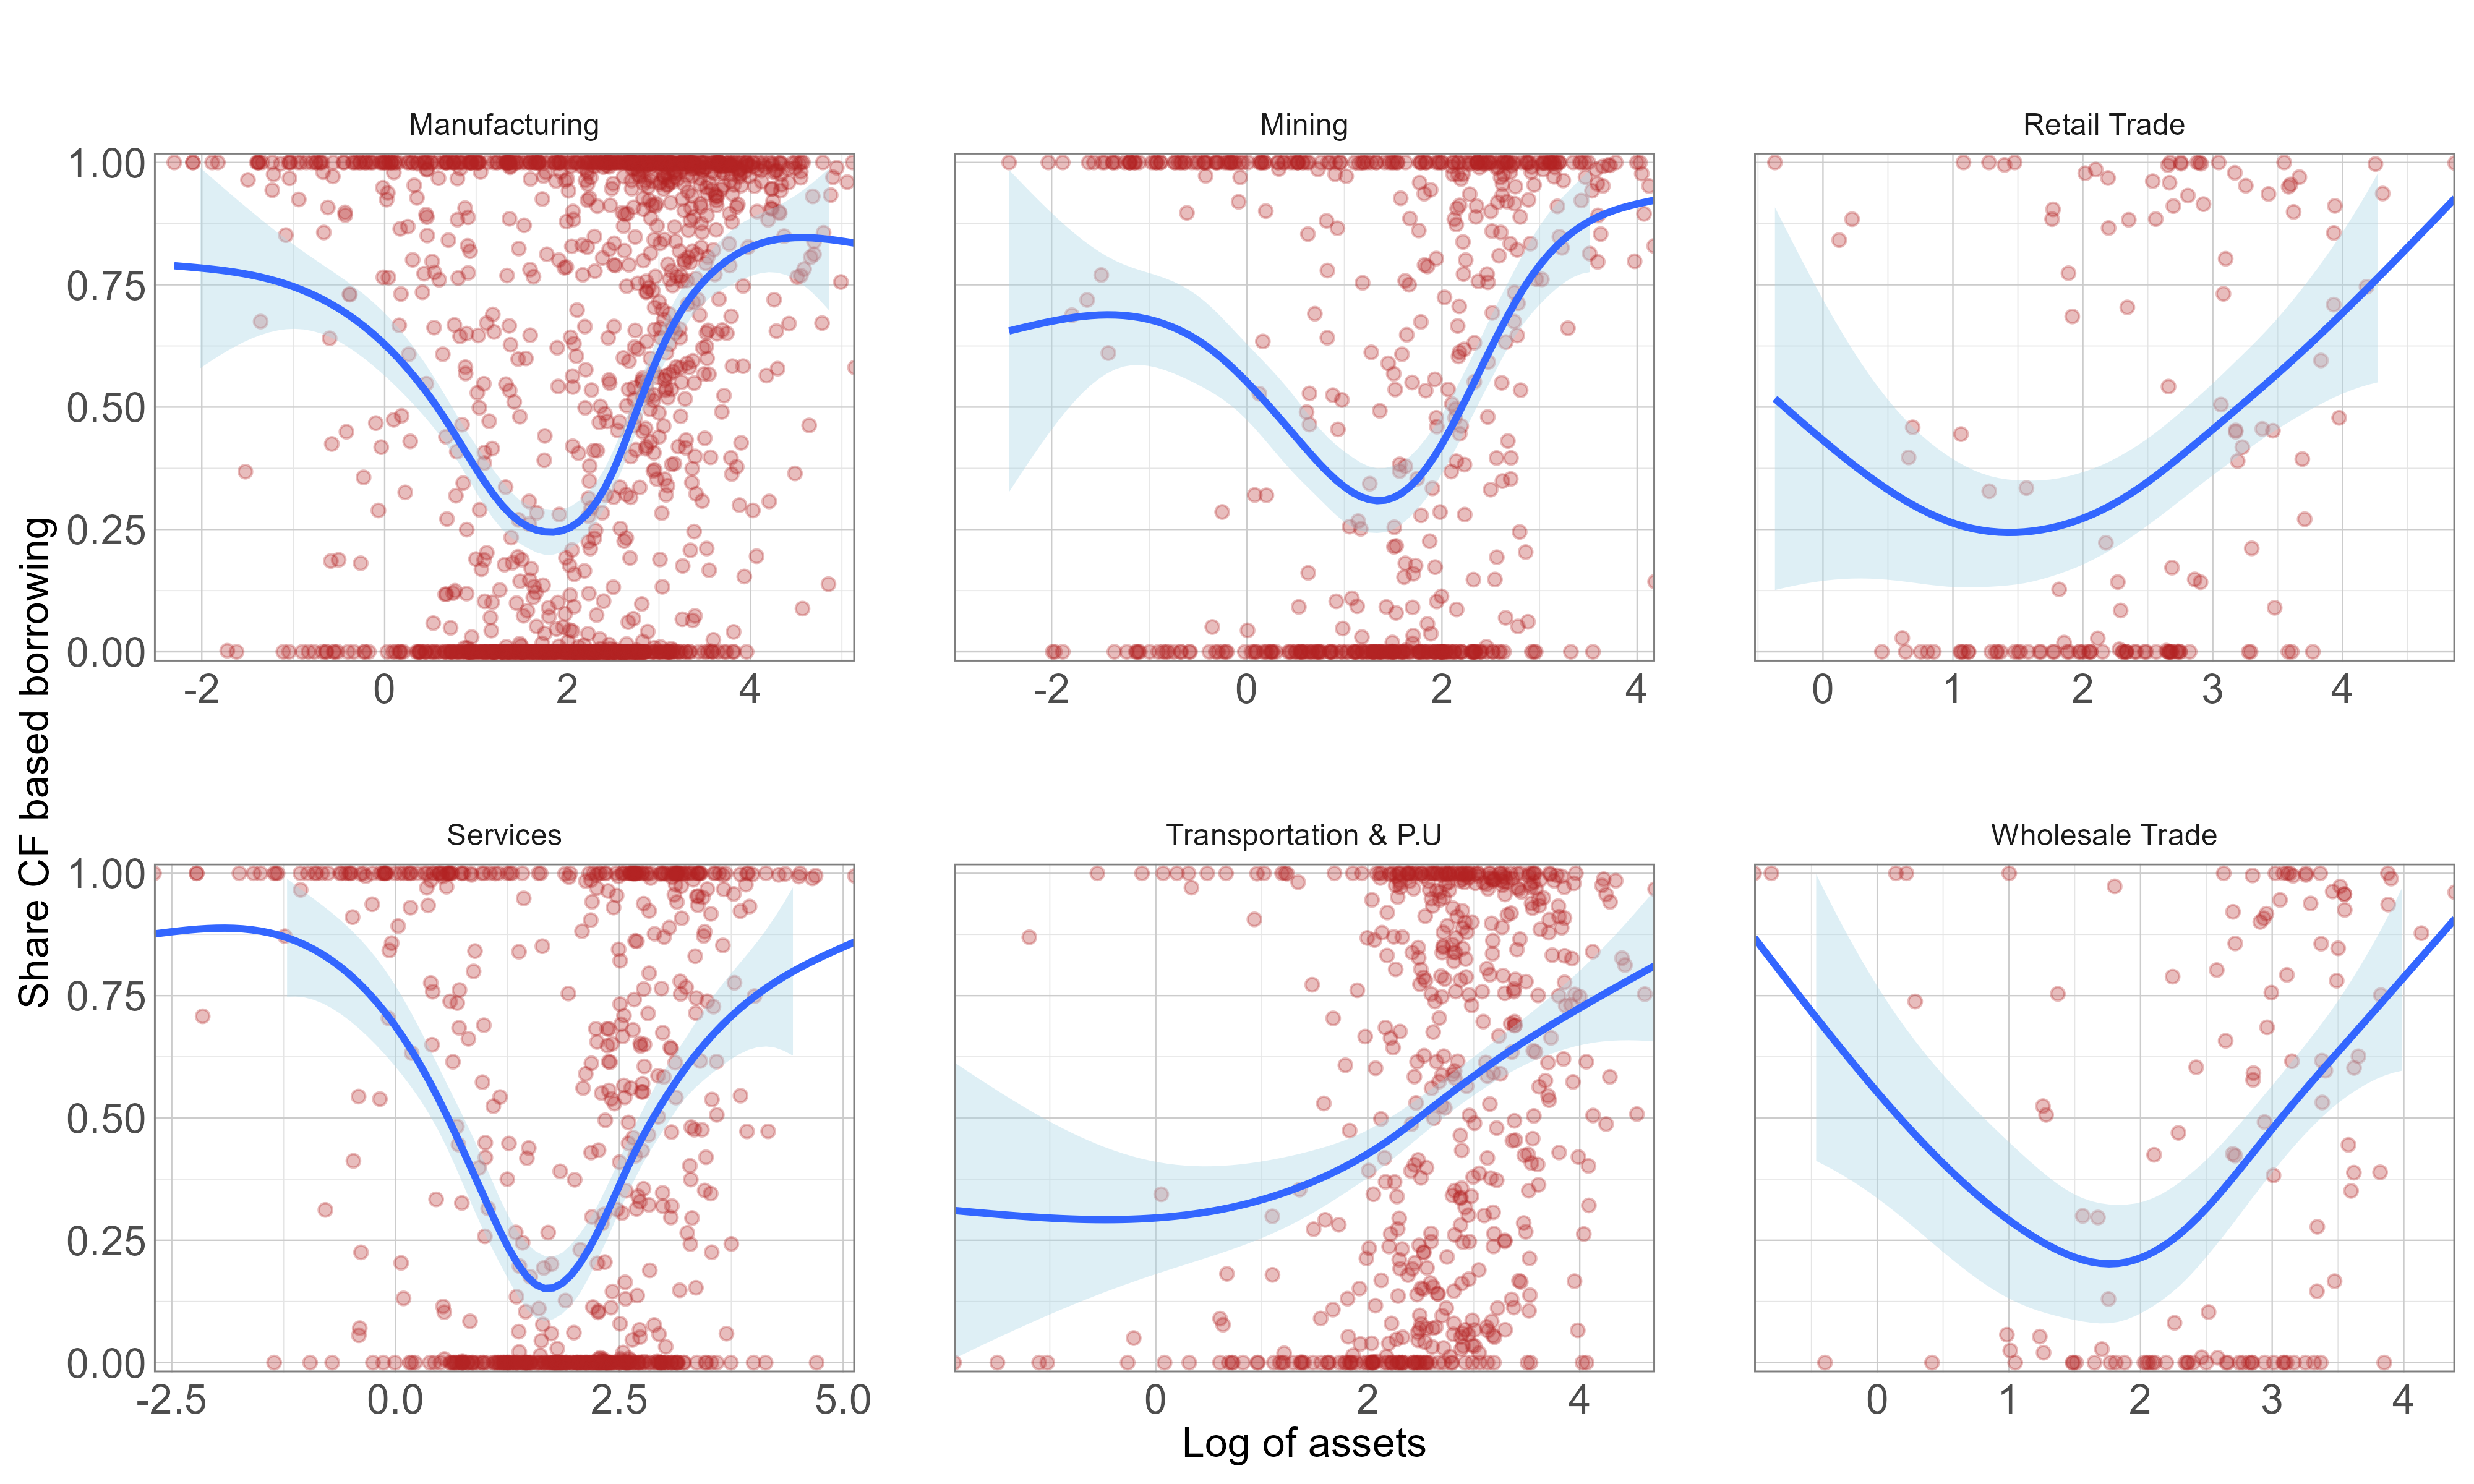
\includegraphics[width=1 \textwidth]{C:/Users/szjud/OneDrive/Asztali gép/EBCs/CFL-git/Latex codes/Plots/smoothy1.png}
\end{figure} \noindent 
\begin{center}
\hyperlink{smoothy}{\beamerreturnbutton{back}} \hspace{5mm}
\end{center}

\end{frame}

%------------------------------------------------
\begin{frame}[label=multi]
\frametitle{CFL share against asset and listing age}

\begin{table}[ht]
\centering
\scalebox{0.7}{%
\begin{tabular}{rrrrr}
  \multicolumn{5}{l}{\textbf{CF share} (share of CFL in total debt)}\\
  \hline
   & Coeff & Std. Error & t value & Pr($>$ $|$t$|$) \\ 
  \hline
  \textit{const.} & 0.5465 & 0.2060 & 2.65 & 0.0081 \\  
  Log assets & -0.1519 & 0.0308 & -4.93 & 0.0000 \\ 
  (Log assets)$^2$ & 0.0644 & 0.0076 & 8.47 & 0.0000 \\ 
  Log age &  -0.2305 & 0.1113 & -2.07 & 0.0386  \\ 
  (Log age)$^2$ & 0.0592 & 0.0223 & 2.65 & 0.0081  \\ 
  \hline
  \multicolumn{5}{l}{\textit{Controls}: Sector, Credit Rating  \hspace{5mm}$n = 1019$, $R^2 = 0.15$ }\\
  \hline
\end{tabular}}

\end{table}

\begin{center}
\hyperlink{smoothy}{\beamerreturnbutton{back}} \hspace{5mm}
\end{center}

\end{frame}

%------------------------------------------------
\begin{frame}[label=Sic CFL] 
\frametitle{CFL reliance across sectors}
\begin{figure} [H]
\centering
\includegraphics[width=1.1 \textwidth]{C:/Users/szjud/OneDrive/Asztali gép/EBCs/CFL-git/Latex codes/Plots/SIC_bars.png}
\end{figure} \noindent 
\begin{center}
\hyperlink{reasons}{\beamerreturnbutton{back}} \hspace{5mm}
\end{center}
\end{frame}


\end{document}
